\documentclass[10pt,a4paper]{article}
\usepackage[margin=0.8in]{geometry}
\usepackage{graphicx}
\usepackage[hidelinks]{hyperref}
\graphicspath{{../data/}{data/}{./}}
\setlength{\parindent}{0pt}
\setlength{\parskip}{4pt}
\pagestyle{empty}

\begin{document}

{\large\textbf{Track A: Flow features of ICMP, TCP and UDP traffic in a Mininet topology}}\\
Name: Dhruv Gupta \quad ID: \textbf{2023A7PS0551P}\\
Repository: \url{https://github.com/codeExplorer7007/mininet-sop}

\textbf{1. Goal.}
Build a small emulated network, capture packet traces for three traffic types (ICMP, TCP, UDP), extract simple per-flow features, and report how the traffic types differ.

\textbf{2. Method.}
Everything ran in an Ubuntu 26.04 VM (VirtualBox) with Mininet. The topology (\texttt{topo.py}) has three hosts and one Open vSwitch in bridge mode (\texttt{OVSBridge}, no controller). Each host link is shaped to 10~Mbit/s with 5~ms delay using \texttt{TCLink}. From h1 to h2 I ran (\texttt{run\_experiment.py}): ICMP (\texttt{ping -c 100 -i 0.2}), TCP bulk (\texttt{iperf3 -t 10}) and UDP (\texttt{iperf3 -u -b 5M -t 10}). Each test was captured with \texttt{tcpdump} on h2's interface into its own pcap. The whole set was repeated 5 times with a fresh network each time (15 captures).
\texttt{features.py} (scapy) groups IP packets into unidirectional flows by 5-tuple (src, dst, sport, dport, protocol) and computes packet count, bytes, mean/std/max packet size, duration, mean inter-arrival time (IAT) and rates. For the comparison I use the main client-to-server flow of each capture (the one with the expected protocol and the most packets) and report mean $\pm$ standard deviation over the 5 runs. All pcaps, logs, the exact commands (\texttt{COMMANDS.md}) and Wireshark screenshots are in the repository.

\textbf{3. Results.}

\begin{center}
\small
\begin{tabular}{|l|r|r|r|r|r|}
\hline
Traffic & Packets & Mean size (B) & Mean IAT (ms) & Duration (s) & Rate (Mbit/s) \\
\hline
ICMP & $100 \pm 0$ & $98.0 \pm 0.0$ & $306 \pm 49$ & $30.3 \pm 4.9$ & $0.003$ \\
TCP  & $3826 \pm 436$ & $2787 \pm 13$ & $3.0 \pm 0.5$ & $11.5 \pm 0.7$ & $7.45 \pm 1.08$ \\
UDP  & $4319 \pm 1$ & $1489.7 \pm 0.0$ & $2.4 \pm 0.1$ & $10.3 \pm 0.3$ & $5.00 \pm 0.16$ \\
\hline
\end{tabular}
\end{center}

\begin{center}
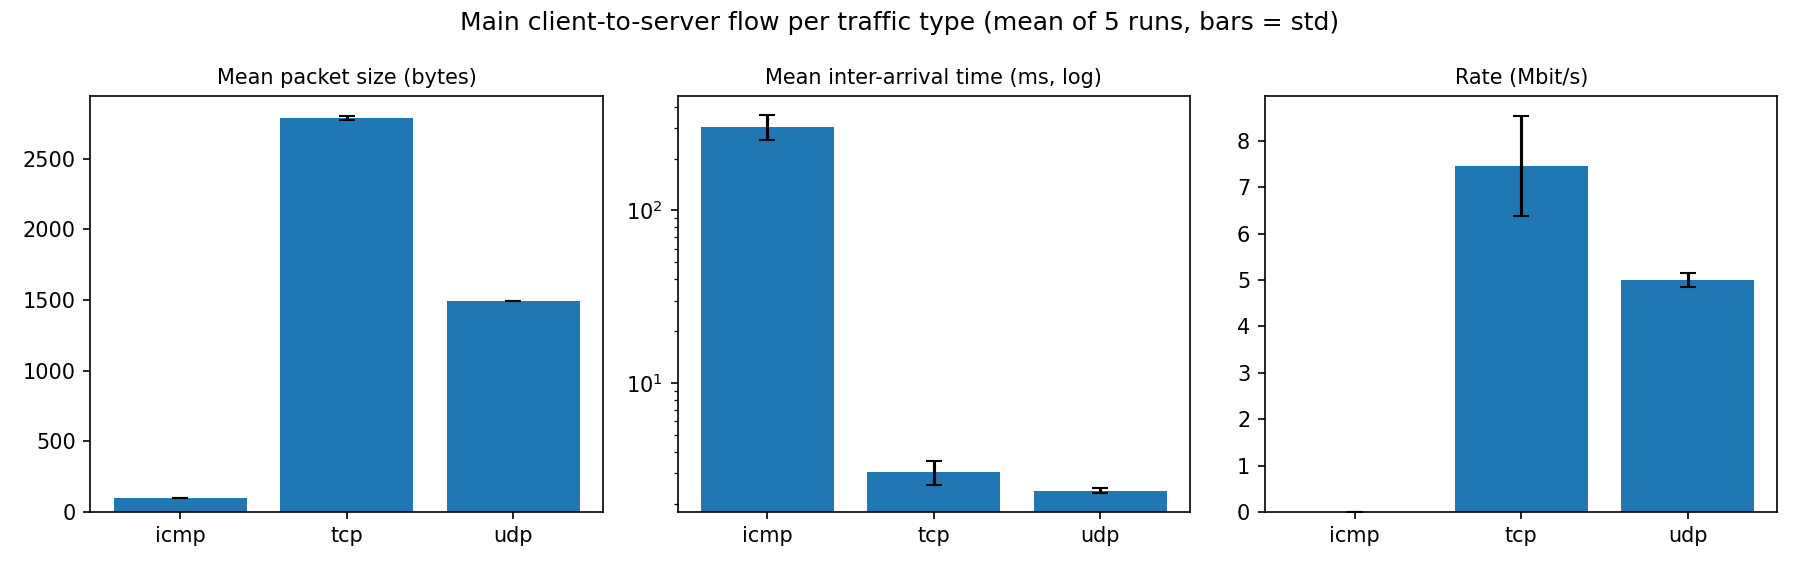
\includegraphics[width=0.97\textwidth]{features_plot.png}
\end{center}

Observations:
(i)~Packet size separates the three types most clearly: ICMP is small and fixed (98 B including the Ethernet header), UDP is a constant 1490 B, and TCP data packets are large.
(ii)~UDP is the most regular. Its rate matches the 5~Mbit/s I requested and varies little between runs, since UDP does not react to the network. TCP's rate varies more (std 1.08~Mbit/s) and stayed below the 10~Mbit/s link capacity (mean 7.45); the iperf3 log of my first, single-run attempt agrees (8.70 sender / 6.85 receiver, \texttt{data/pilot/}).
(iii)~One iperf3 TCP run is more than one flow. In \texttt{tcp\_run1} Wireshark shows two connections: a control connection (36 packets, 3~kB) and the data stream (8,307 packets, 12~MB, both directions), and the reverse ACK flow of the data stream has tiny packets (about 65 B). This is why a flow must be defined by its 5-tuple and direction.
(iv)~ICMP timing was irregular. Over the 5 runs the median gap between requests was 207--282~ms (requested: 200~ms), and every run had stalls, with a maximum gap of 702--1244~ms (\texttt{icmp\_gaps.py}). These stalls pull the mean IAT in the table (306~ms) above the typical gap, so I treated the mean IAT as noisy. I did not test the cause; VM scheduling or host load are possible.

\textbf{4. Main limitation.}
All results come from one emulated network inside one VM, so the numbers describe this setup and not a real network. The clearest sign is TCP packet size: the mean is 2787~B and the maximum above 4000~B, more than the 1500~B Ethernet MTU. This is probably segmentation offload merging packets before tcpdump sees them (a hypothesis I did not test), so a physical switch would not see TCP packets of this size. Other limits: only 5 runs and a single client/server pair; synthetic traffic (iperf3, ping); TCP throughput variability and a flow duration longer than the 10~s test are unexplained; VM scheduling may add timing noise; and the switch is a plain bridge with no controller, so nothing here says anything about SDN control. A first single-run attempt was discarded because its TCP capture also contained UDP packets (the capture process had not finished), and is kept in \texttt{data/pilot/}.

\textbf{5. Week two.}
I would make the network programmable by replacing the plain bridge with an OpenFlow controller (Ryu) or a P4 switch on BMv2, and add more traffic types (HTTP downloads, DNS). I would run more repetitions and report confidence intervals, test the offload hypothesis by turning offload off with \texttt{ethtool}, find out what causes the long ICMP stalls (for example by repeating the test with other load on the host stopped), and then compute the features from only the first few packets of each flow to see whether the traffic types can still be told apart.

\textbf{6. Randomness and AI use.}
No randomness is used in the experiment or the analysis, so a seed is not needed; had I used one, it would be 51 (last two digits of my ID). I used Claude (Anthropic) for: guidance on setting up VirtualBox, Ubuntu and Mininet; drafting the first versions of \texttt{topo.py}, \texttt{run\_experiment.py}, \texttt{features.py} and \texttt{icmp\_gaps.py}; debugging errors (permissions, stale Mininet interfaces, a contaminated capture); and a first draft of this report, which I reviewed and edited. I ran all commands myself and made these choices: 5 repeats, a table plus one plot, and keeping the link settings fixed. Where I got stuck is described in \texttt{NOTES.md}.

\end{document}
